\documentclass{article}
\usepackage{graphicx}
\usepackage{amsmath}
\usepackage{siunitx}
\usepackage{tikz}
\usepackage{pgfplots}
\usepackage{float}
\usepackage{circuitikz}
\usepackage{subcaption}
\title{Bode Plot Analysis of Cascaded RC Low-Pass Filters}
\author{EE24BTECH11048-NITHIN.K\\EE24BTECH11021-ESHAN RAY}
\date{\today}

\begin{document}

\maketitle

\section{Introduction}
An RC low-pass filter is a fundamental electronic circuit that allows low-frequency signals to pass while attenuating high-frequency components. Cascading multiple RC filters improves the roll-off characteristics, making the filter more effective in suppressing unwanted high-frequency noise.
\section{Materials and Apparatus Required}
\begin{itemize}
    \item 3 Resistors (1k$\Omega$ used)
    \item 3 Capacitors (1$\mu$F used)
    \item Breadboard
    \item Function Generator
    \item Oscilloscope
\end{itemize}
\section{Procedure}
\begin{enumerate}
    \item Assemble the circuit as shown in the below figure.
    \item Apply input \( V_{in} \) from a function generator.
    \item Measure voltage across each stage.
    \item Record phase difference for multiple frequencies.
    \item Repeat for 1-stage, 2-stage, and 3-stage filters.
    \item Compare theoretical and experimental results.
\end{enumerate}
\begin{figure}[H]
    \centering
    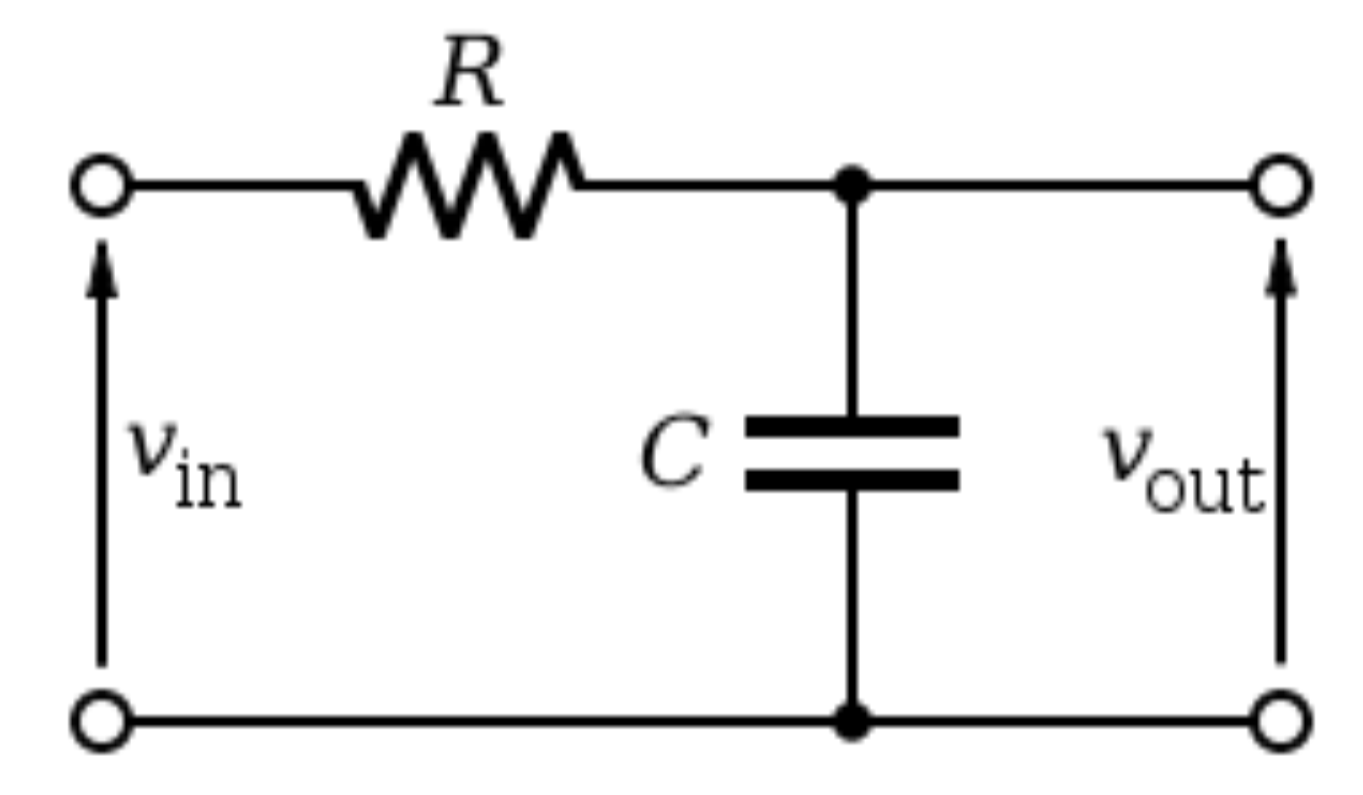
\includegraphics[width=0.5\textwidth]{figs/circ1.png}
    \caption{RC circuit}
\end{figure}
\begin{figure}[h]
    \centering
    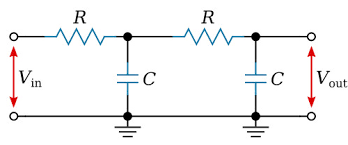
\includegraphics[width=0.7\textwidth]{figs/circ2.png}
    \caption{RC cascaded with another RC}
\end{figure}

\begin{figure}[H]
    \centering
    \begin{circuitikz} 
        \draw
        (0,2) to[short, *-] (0,2) node[circle, fill, inner sep=1pt] {}
        to[R=$R$] (2,2) to[R=$R$] (4,2) to[R=$R$] (6,2)
        to[short, -*] (7,2) to[short, -*] (7,0) node[circle, fill, inner sep=1pt] {}
        (0,2) to[short, -*] (0,0)
        (2,2) to[short, *-] (2,1.5) to[C=$C$] (2,0) 
        (4,2) to[short, *-] (4,1.5) to[C=$C$] (4,0) 
        (6,2) to[short, *-] (6,1.5) to[C=$C$] (6,0)
        (0,0) to[short] (4,0) to[short] (6,0)
        (6,0) to[short, -*] (7,0);
        \node[left] at (0,2) {$V_{in}$};
        \node[right] at (7,2) {$V_{out}$};
    \end{circuitikz}
    \caption{RC cascades with 2 RCs}
\end{figure}
\section{Theory}
A single-stage RC low-pass filter consists of a resistor (R) and a capacitor (C) in series, with the output taken across the capacitor. The transfer function is given by:
\begin{equation}
H(s) = \frac{1}{1 + sRC}
\end{equation}
where \( s = j\omega \) and \( \omega \) is the angular frequency.

The cutoff frequency \( f_c \) is determined as:
\begin{equation}
f_c = \frac{1}{2\pi RC}
\end{equation}

\subsection{Cascading RC Filters}
Cascading multiple RC filters increases the overall roll-off rate. The roll-off for each stage is approximately \(-20\) dB/decade:
\begin{itemize}
    \item \textbf{1-stage:} \(-20\) dB/decade
    \item \textbf{2-stage:} \(-40\) dB/decade
    \item \textbf{3-stage:} \(-60\) dB/decade
\end{itemize}
Each stage provides additional attenuation, making cascaded RC filters effective in audio signal processing and communication systems.


\section{Theory}

The transfer function of a 1-stage RC circuit is given by:

\begin{align*}
    H(s) = \frac{1}{1+sRC}
\end{align*}

where,

\begin{align*}
    s = j\omega.
\end{align*}

Expanding, we get:

\begin{align*}
    H(s) = \frac{1}{\sqrt{1+(\omega RC)^2}} e^{j\theta}
\end{align*}

where,

\begin{align*}
    \theta = -\tan^{-1}(\omega RC).
\end{align*}

Applying logarithm on both sides,

\begin{align*}
    \log H(s) &= \log\left(\frac{1}{\sqrt{1+(\omega RC)^2}} e^{j(-\tan^{-1}(\omega RC))}\right)\\
              &= -\frac{1}{2}\log(1+(\omega RC)^2) - j\tan^{-1}(\omega RC).
\end{align*}

Calculating amplitude gain:

\begin{align*}
    A &= 20 \log\left| H(s) \right|\\
    &= -10 \log(1+(\omega RC)^2).
\end{align*}

This gives the exact equation for the Bode plot of the amplitude gain.

For phase difference,

\begin{align*}
    \theta &= -\tan^{-1}(\omega RC).
\end{align*}

Similarly, the transfer function of a 2-stage RC circuit is given by:

\begin{align*}
    H(s) = \frac{1}{1 + 3sRC + (sRC)^2}.
\end{align*}

Following this, we get:

\begin{align*}
    \log H(s) = -\frac{1}{2} \log \left( (1-(\omega RC)^2)^2 + (3\omega RC)^2 \right) + j \tan^{-1} \left( \frac{-3\omega RC}{1-(\omega RC)^2} \right).
\end{align*}

The transfer function for a 3-stage RC circuit is given as:

\begin{align*}
    H(s) = \frac{1}{(sRC)^3 + 5(sRC)^2 + 6sRC + 1}.
\end{align*}

Following that, we get:

\begin{align*}
    \log H(s) = -\frac{1}{2} \log \left( \left( 1 + 6\omega RC + 5(\omega RC)^2 + (\omega RC)^3 \right)^2 \right) + j \tan^{-1} \left( \frac{-6\omega RC - (\omega RC)^3}{1 + 5(\omega RC)^2} \right).
\end{align*}

\section{Bode Plot Analysis}
The magnitude response for a single-stage RC filter follows:
\begin{equation}
|H(j\omega)| = \frac{1}{\sqrt{1 + (\omega RC)^2}}
\end{equation}
And the phase response is given by:
\begin{equation}
\theta(\omega) = -\tan^{-1}(\omega RC)
\end{equation}

For multiple stages, the overall transfer function is:
\begin{equation}
H_n(s) = \left(\frac{1}{1 + sRC}\right)^n
\end{equation}
where \( n \) is the number of stages.

\begin{figure}[H]
    \centering
    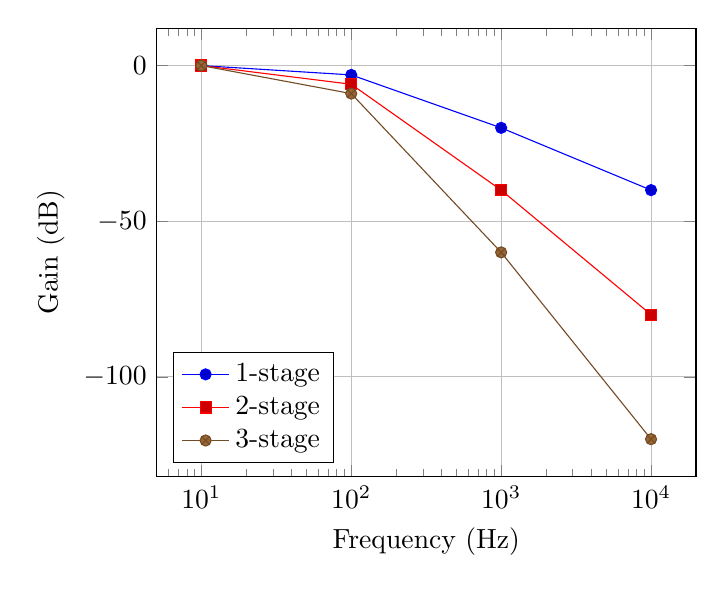
\begin{tikzpicture}
    \begin{semilogxaxis}[
        xlabel={Frequency (Hz)},
        ylabel={Gain (dB)},
        grid=major,
        legend pos=south west
    ]
    \addplot coordinates {(10, 0) (100, -3) (1000, -20) (10000, -40)};
    \addlegendentry{1-stage}
    \addplot coordinates {(10, 0) (100, -6) (1000, -40) (10000, -80)};
    \addlegendentry{2-stage}
    \addplot coordinates {(10, 0) (100, -9) (1000, -60) (10000, -120)};
    \addlegendentry{3-stage}
    \end{semilogxaxis}
    \end{tikzpicture}
    \caption{Bode plot for cascaded RC filters}
\end{figure}
\section{Observations}
\begin{figure}[H]
    \centering
    \begin{subfigure}[b]{0.45\textwidth}
        \centering
        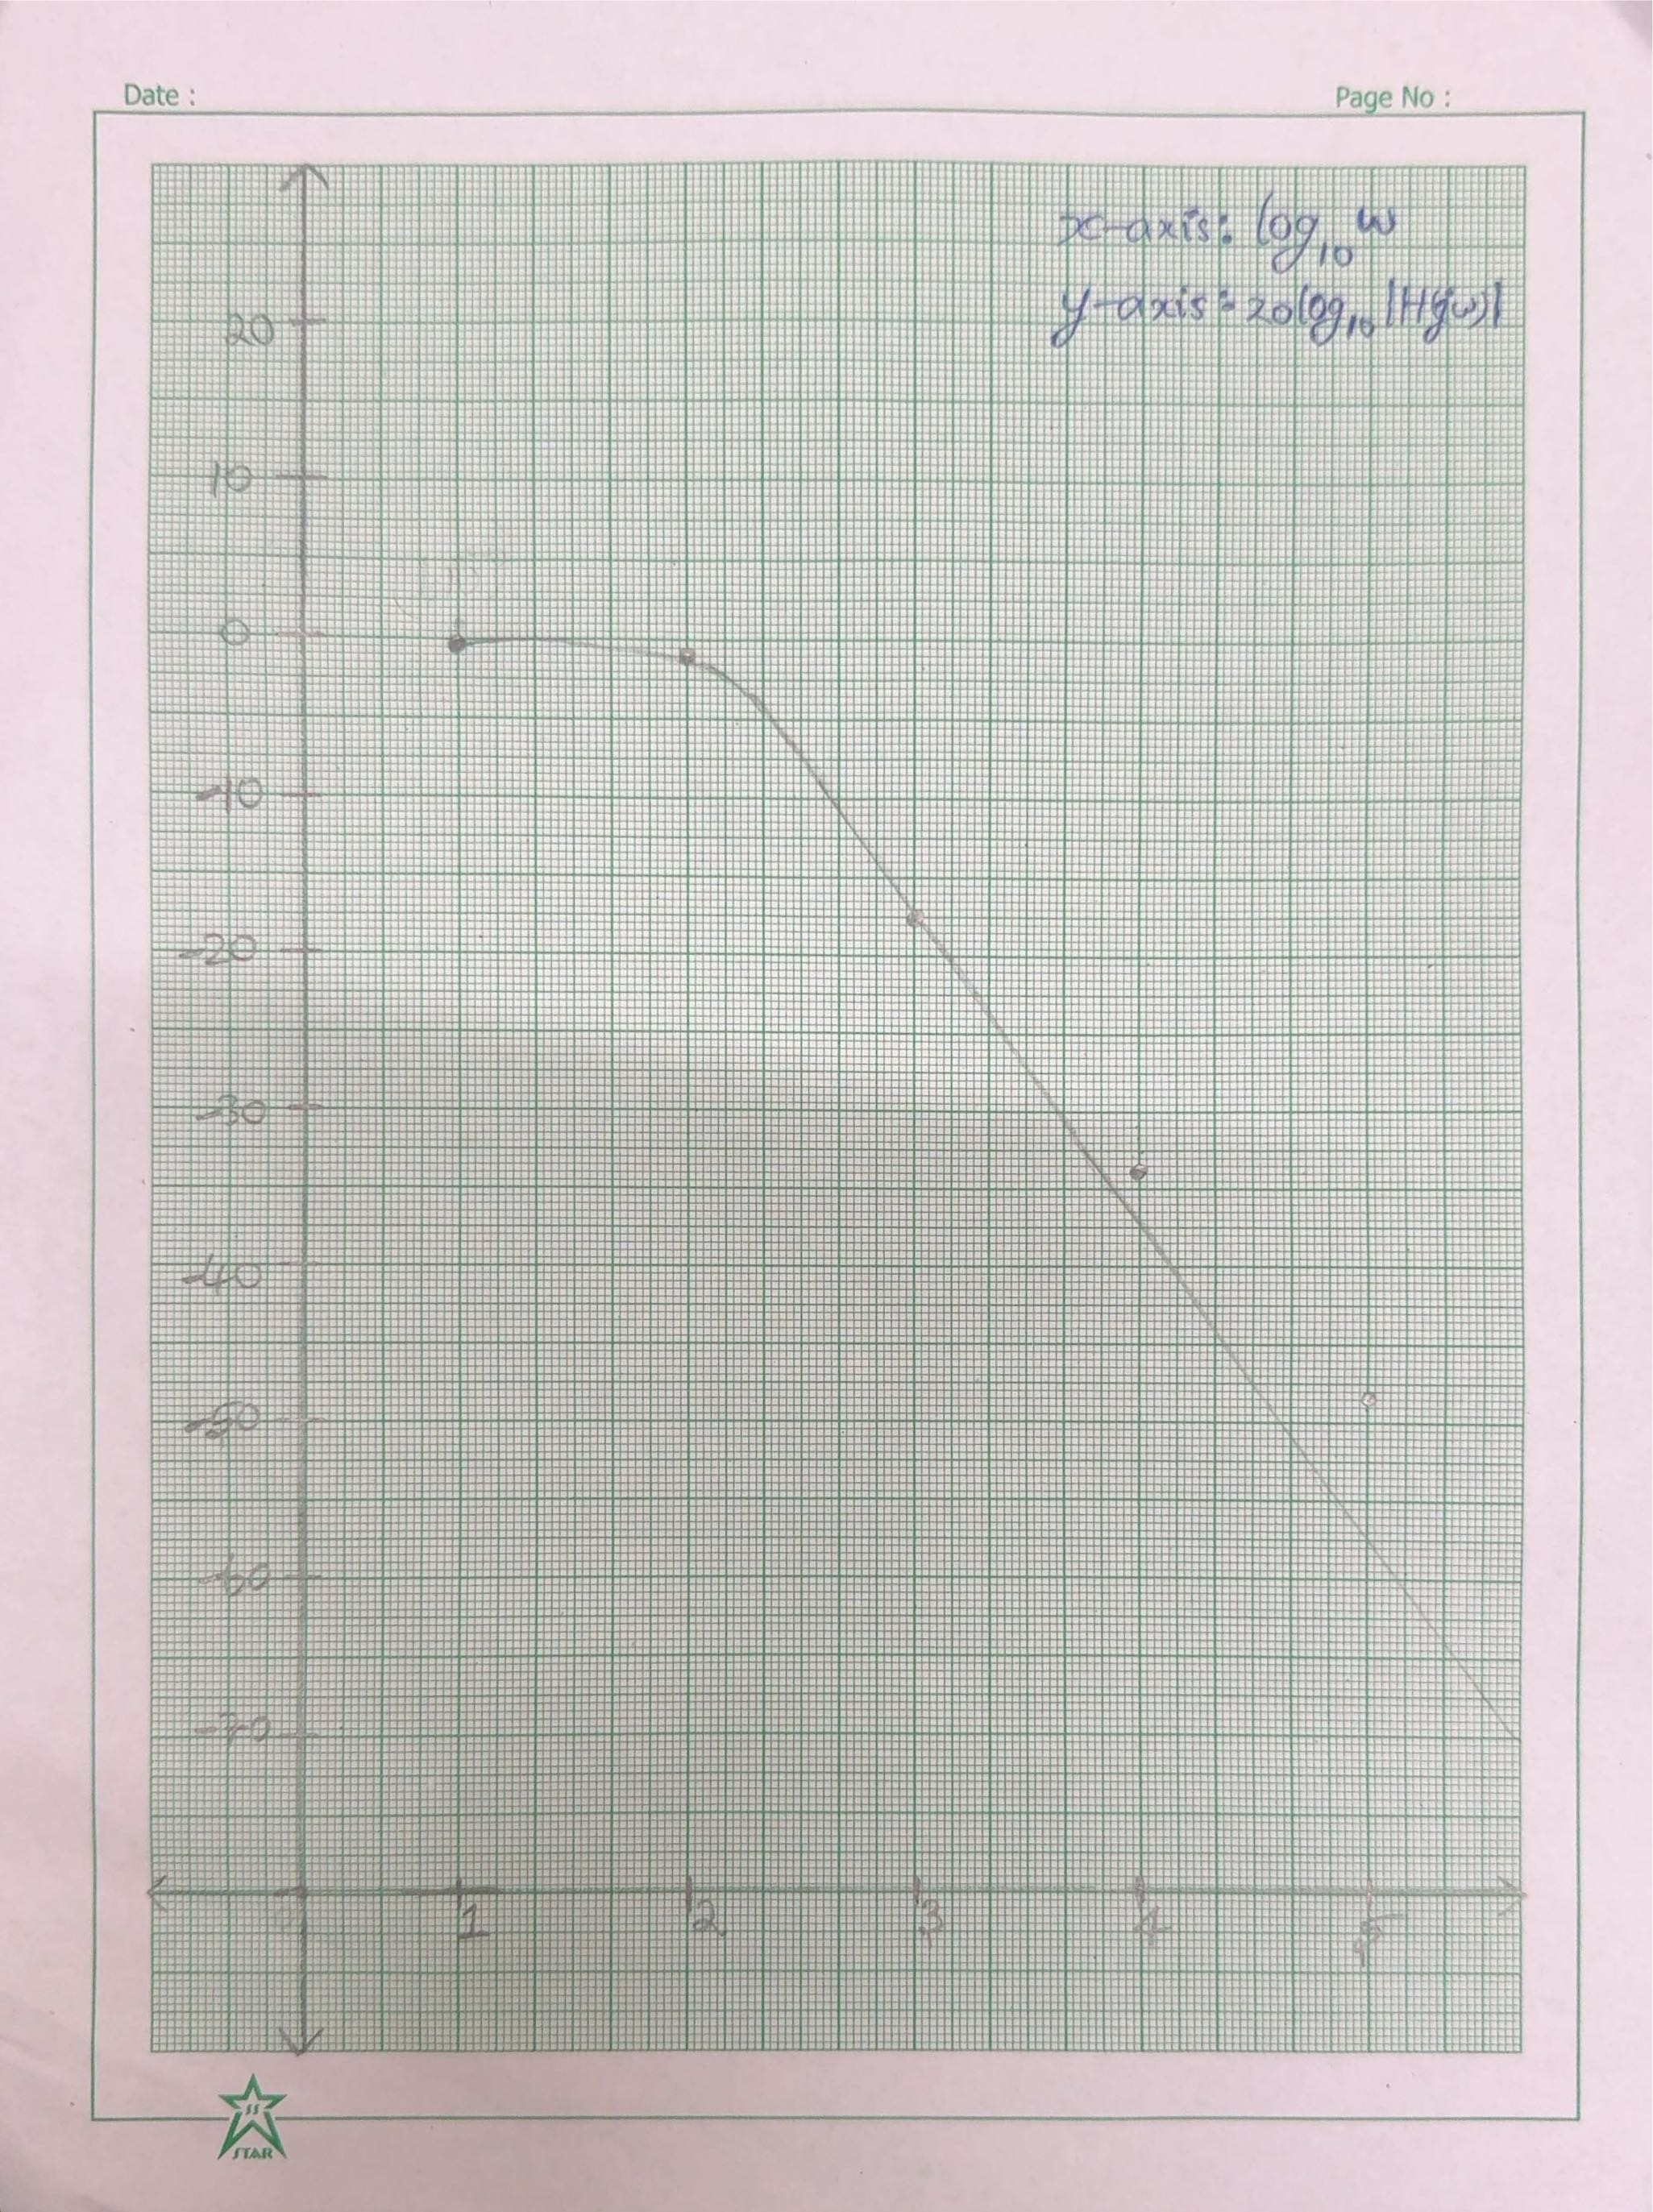
\includegraphics[width=\textwidth]{figs/ampl1.png}
    \end{subfigure}
    \hfill
    \begin{subfigure}[b]{0.45\textwidth}
        \centering
        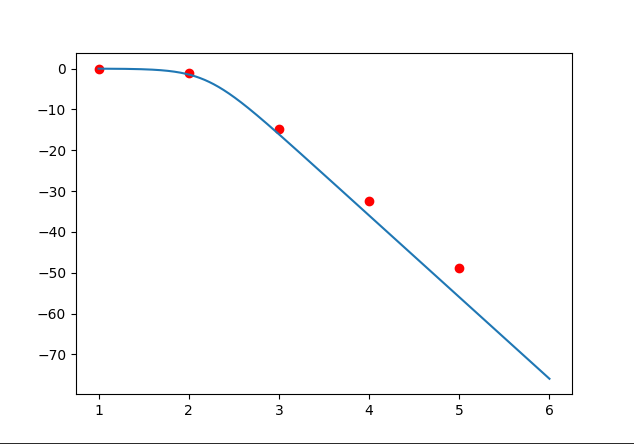
\includegraphics[width=1.7\textwidth]{figs/ampl_1cas.png}
    \end{subfigure}
    
    \caption{Amplitude Plot for RC circuit}
\end{figure}

\begin{figure}[H]
    \centering
    \begin{subfigure}[b]{0.45\textwidth}
        \centering
        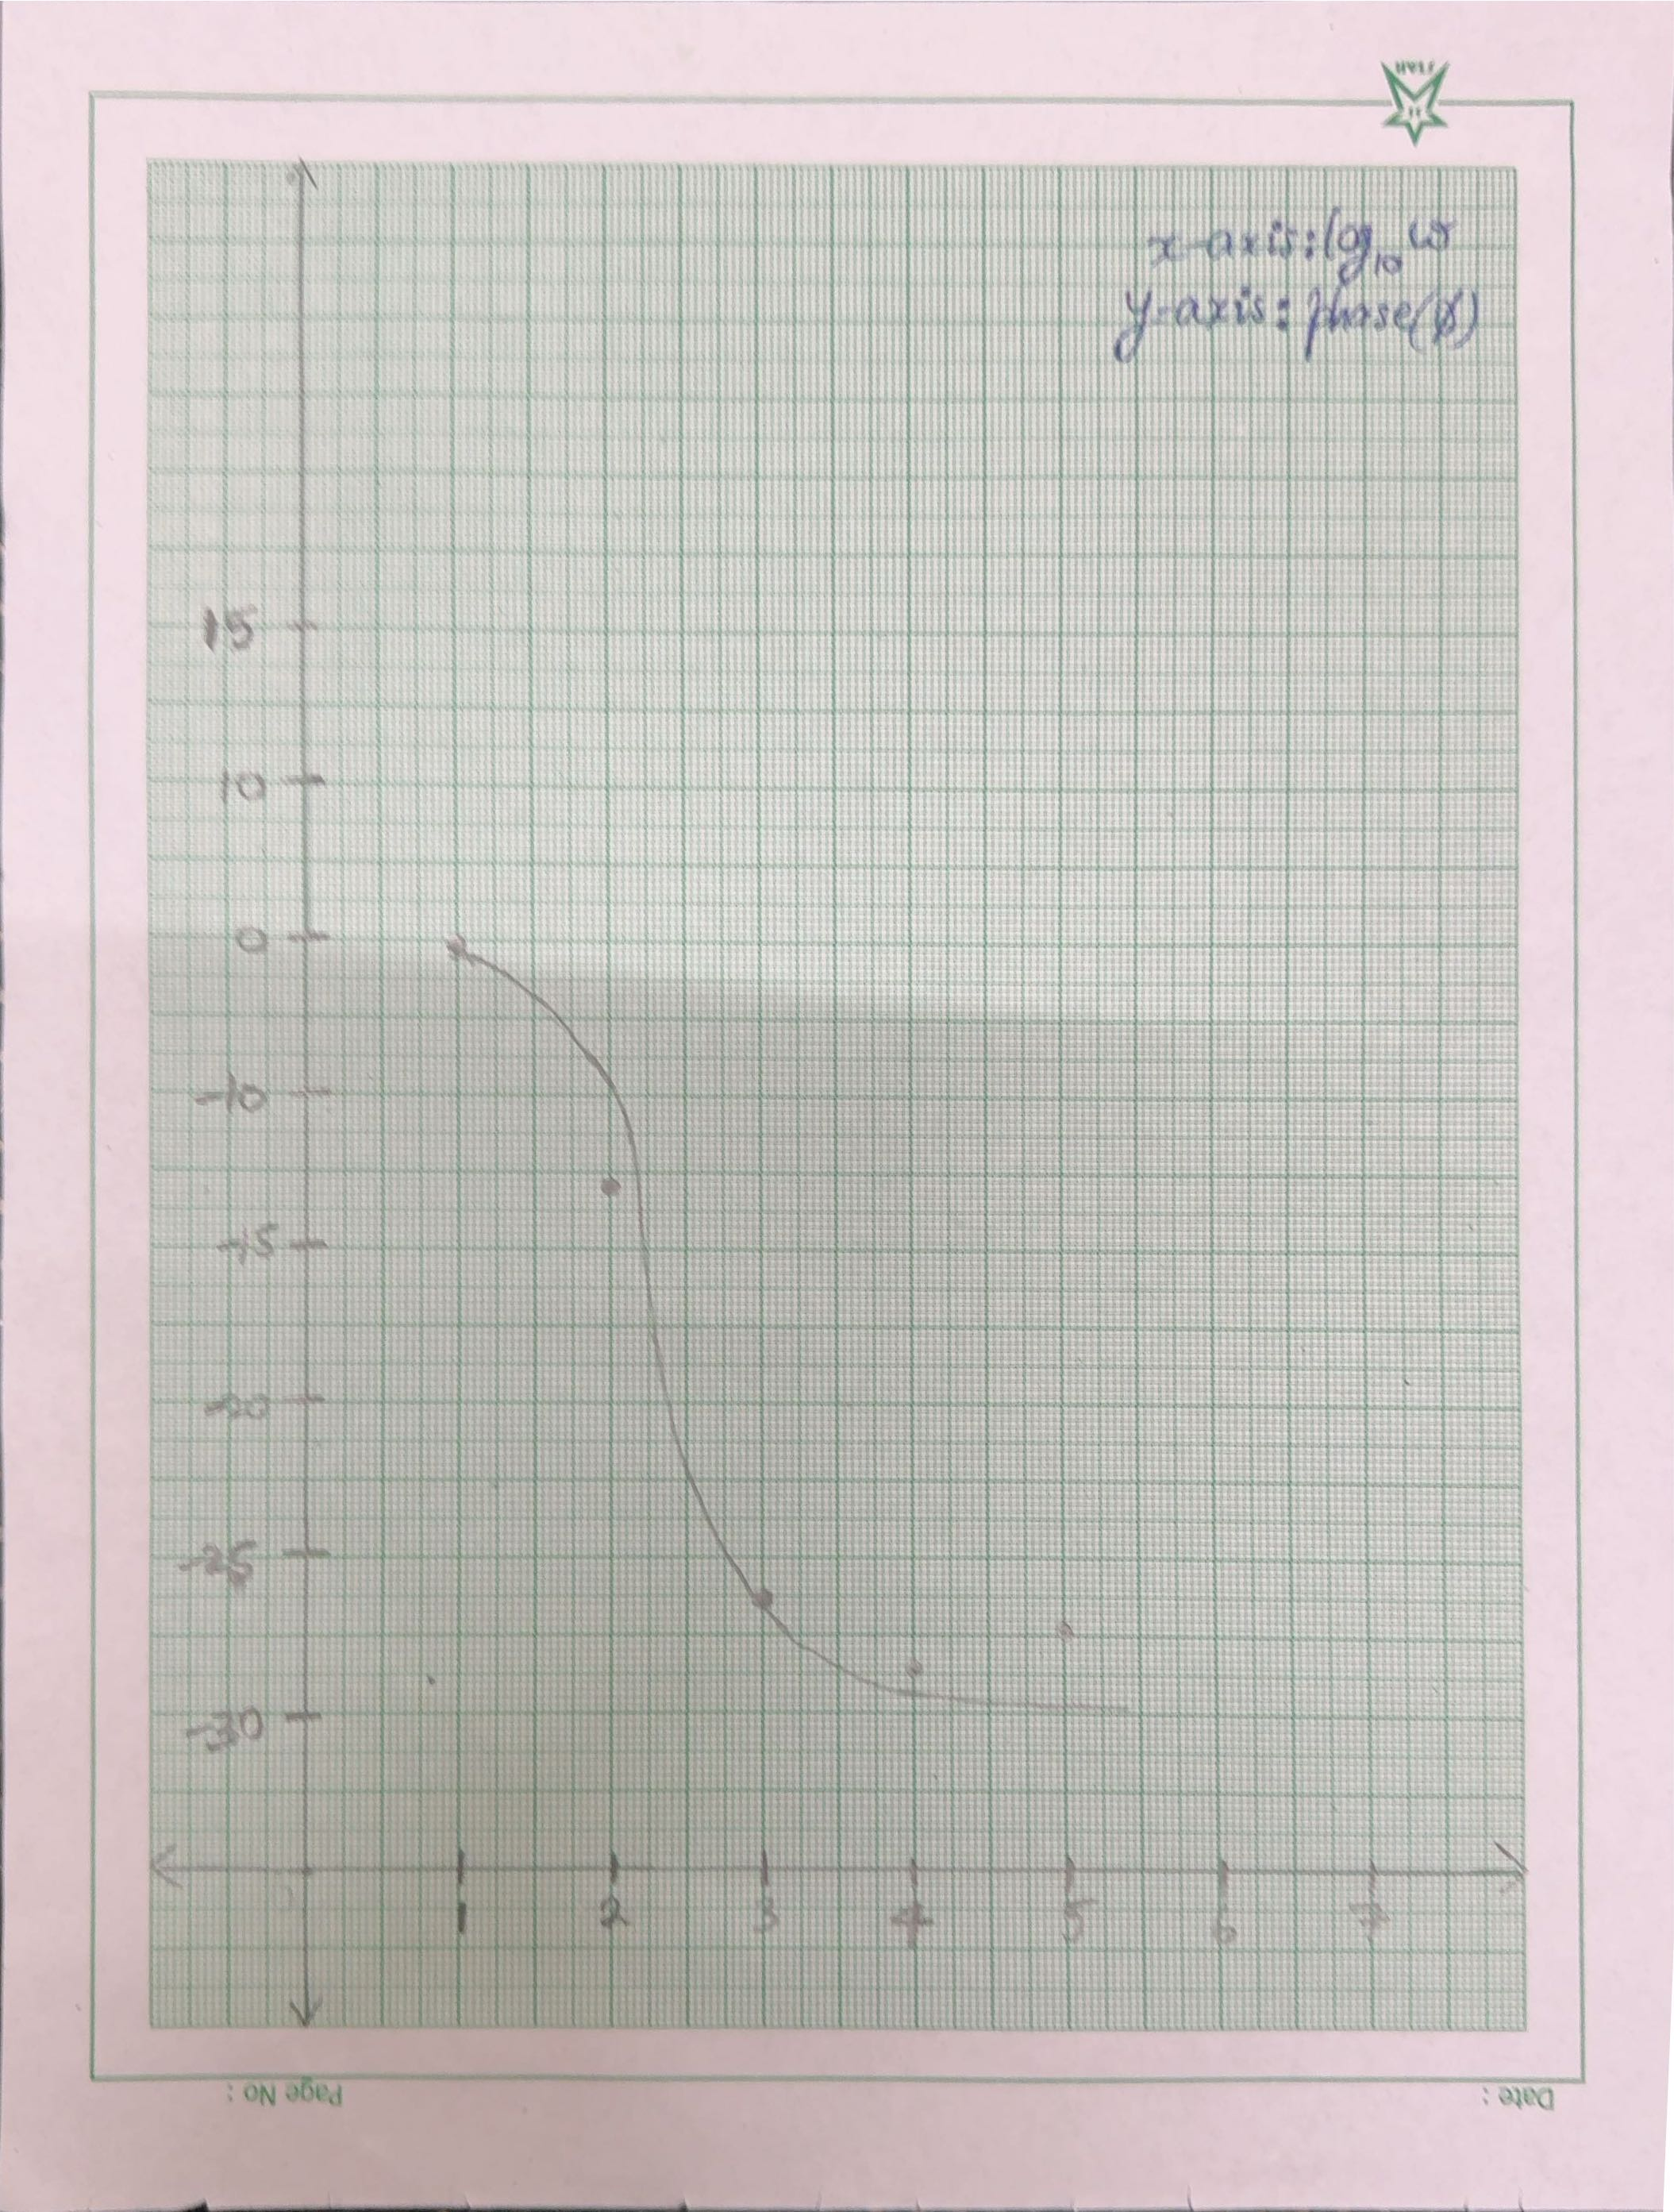
\includegraphics[width=\textwidth]{figs/phase1.png}
    \end{subfigure}
    \hfill
    \begin{subfigure}[b]{0.45\textwidth}
        \centering
        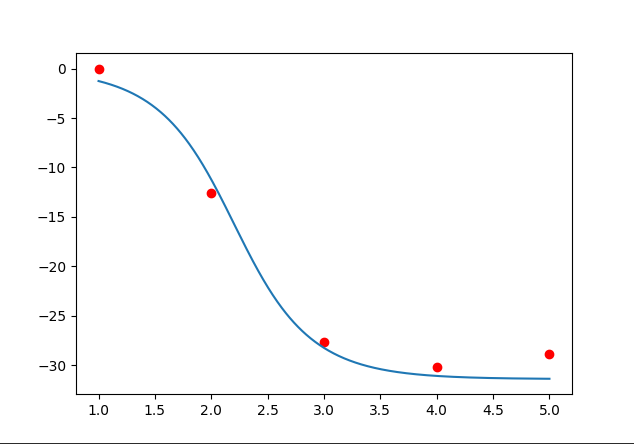
\includegraphics[width=1.7\textwidth]{figs/phase_1cas.png}
    \end{subfigure}
    
    \caption{Phase Plot for RC circuit}
\end{figure}

\begin{figure}[H]
    \centering
    \begin{subfigure}[b]{0.45\textwidth}
        \centering
        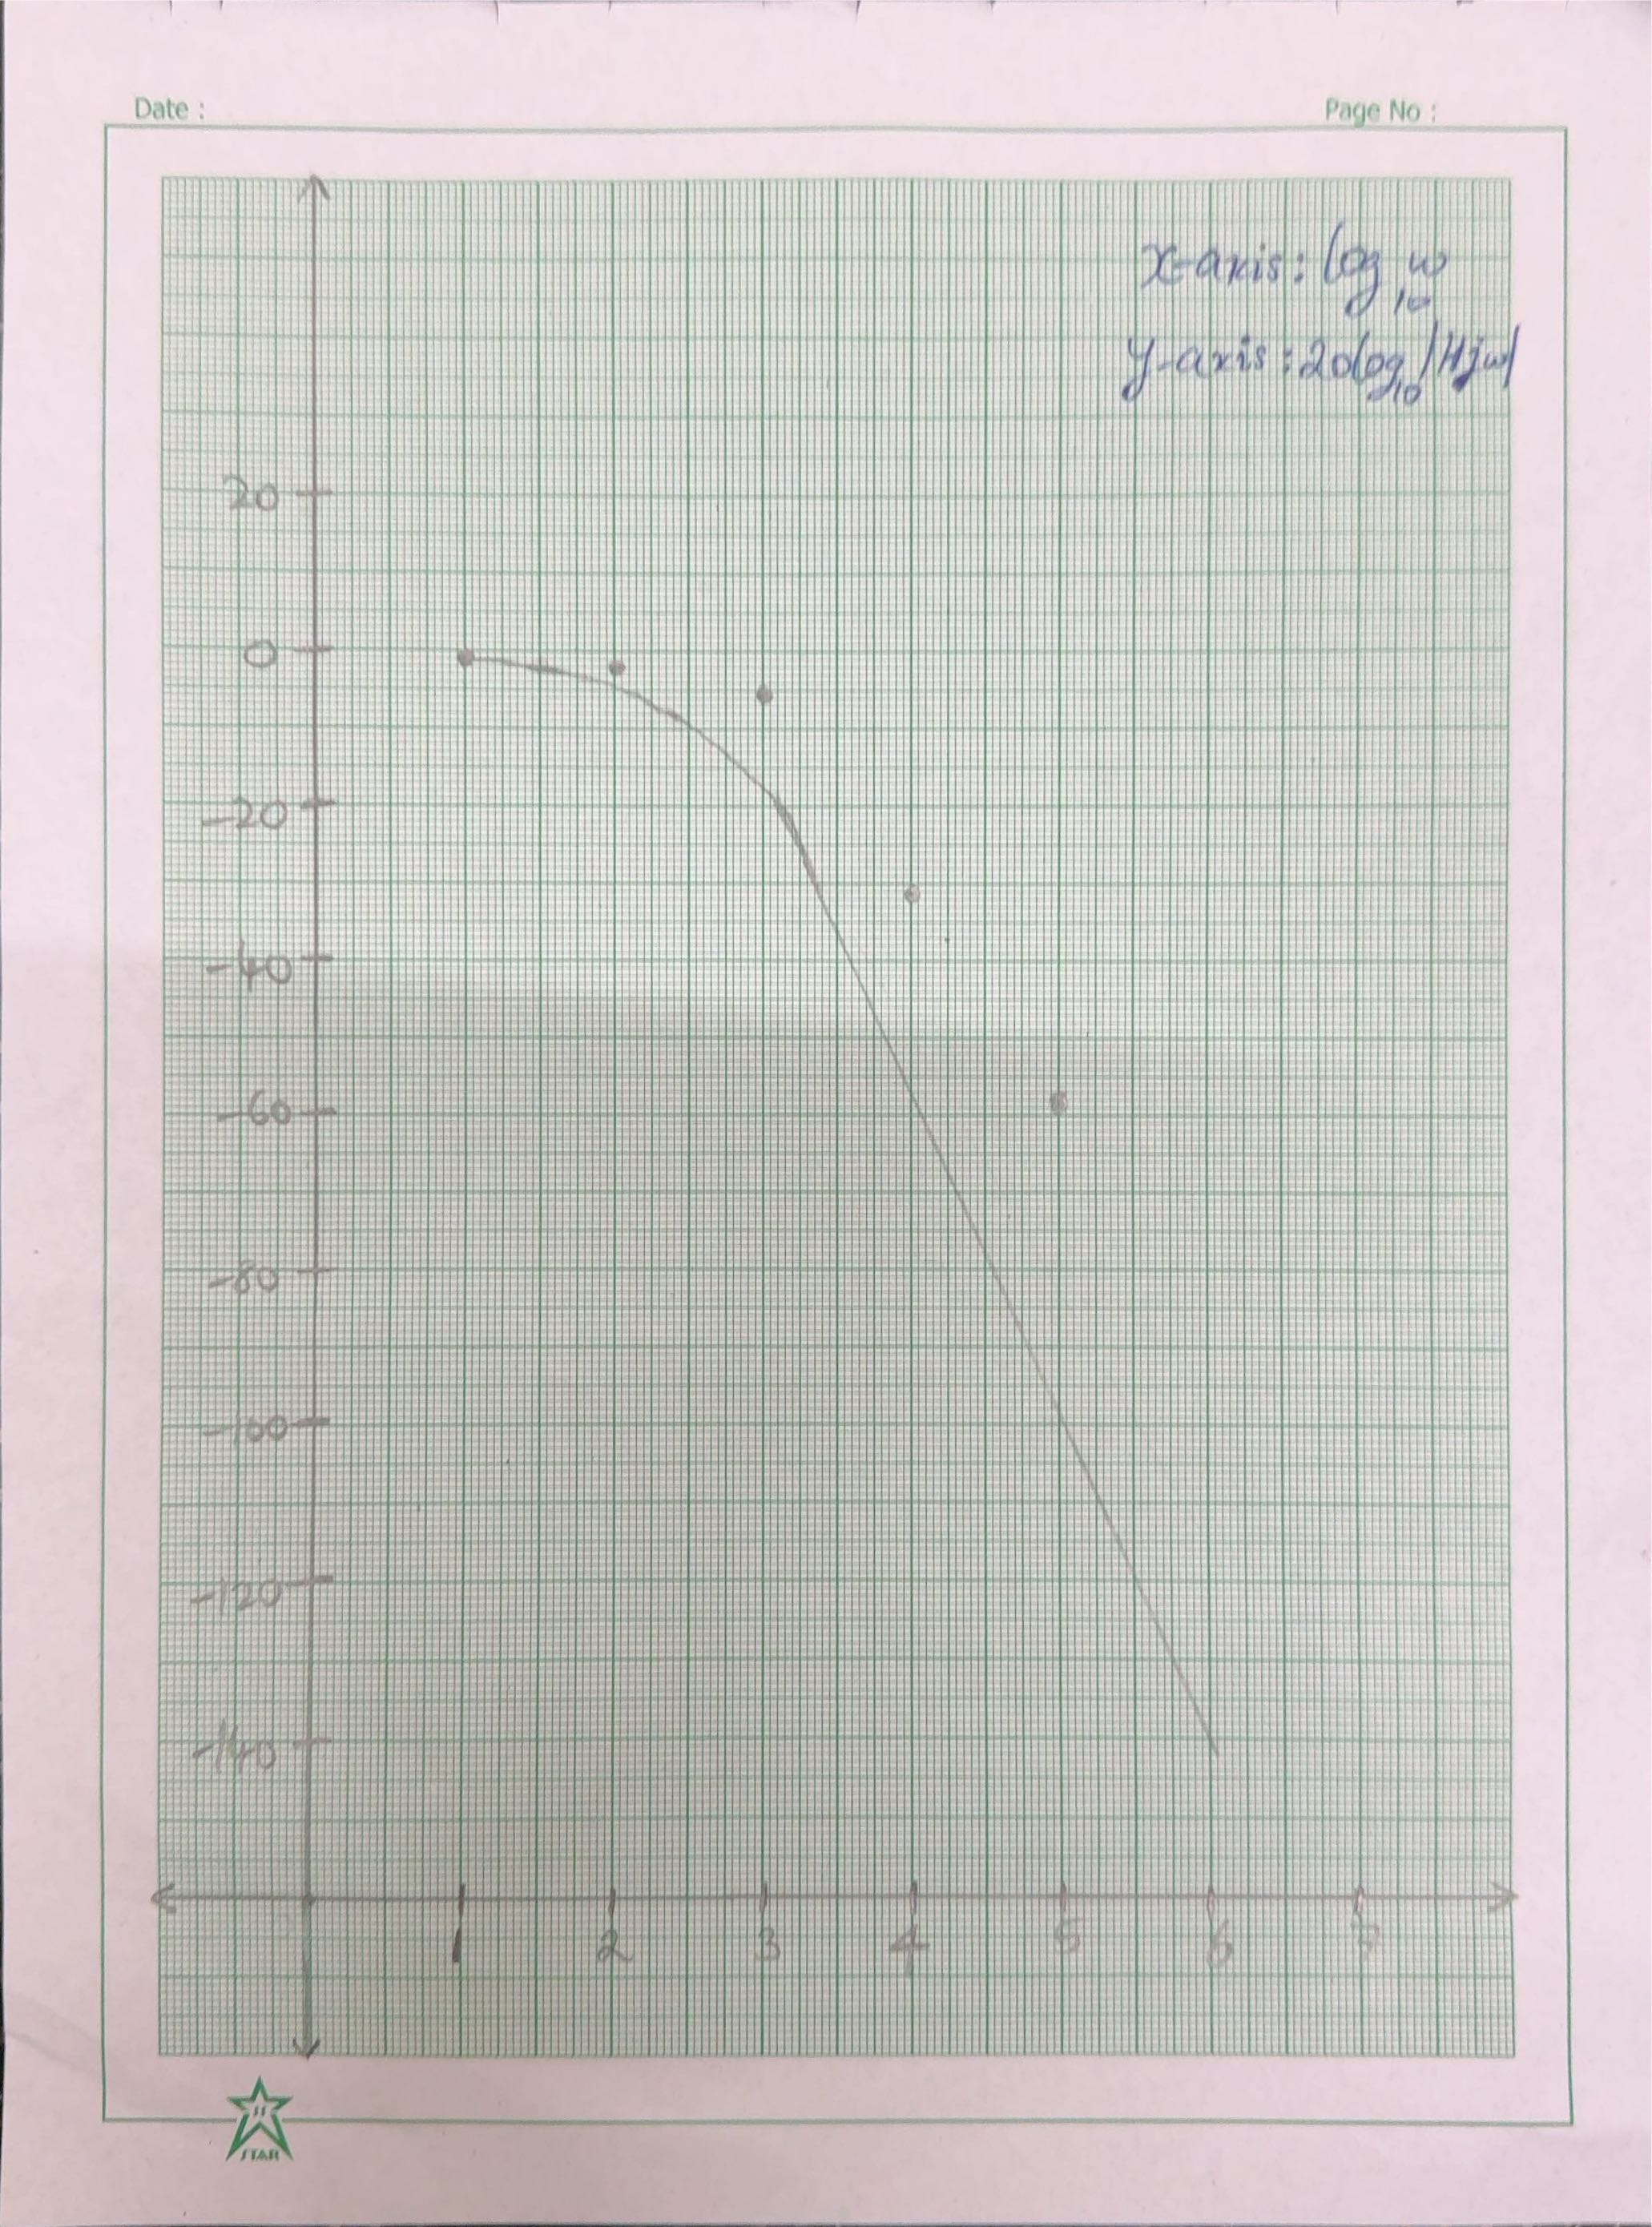
\includegraphics[width=\textwidth]{figs/ampl2.png}
    \end{subfigure}
    \hfill
    \begin{subfigure}[b]{0.45\textwidth}
        \centering
        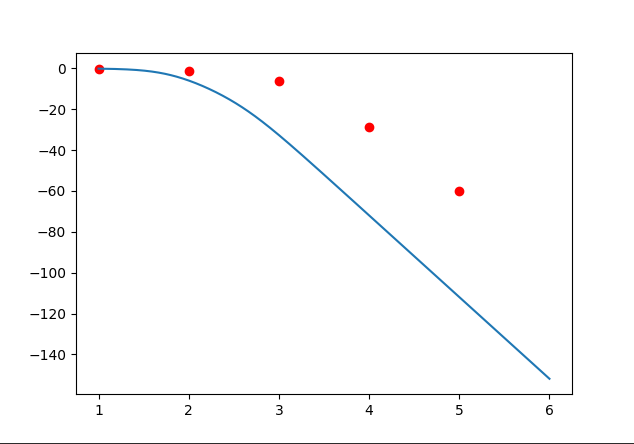
\includegraphics[width=1.7\textwidth]{figs/ampl_2cas.png}
    \end{subfigure}
    
    \caption{Amplitude Plot for 2 cascaded RC circuit}
\end{figure}

\begin{figure}[H]
    \centering
    \begin{subfigure}[b]{0.45\textwidth}
        \centering
        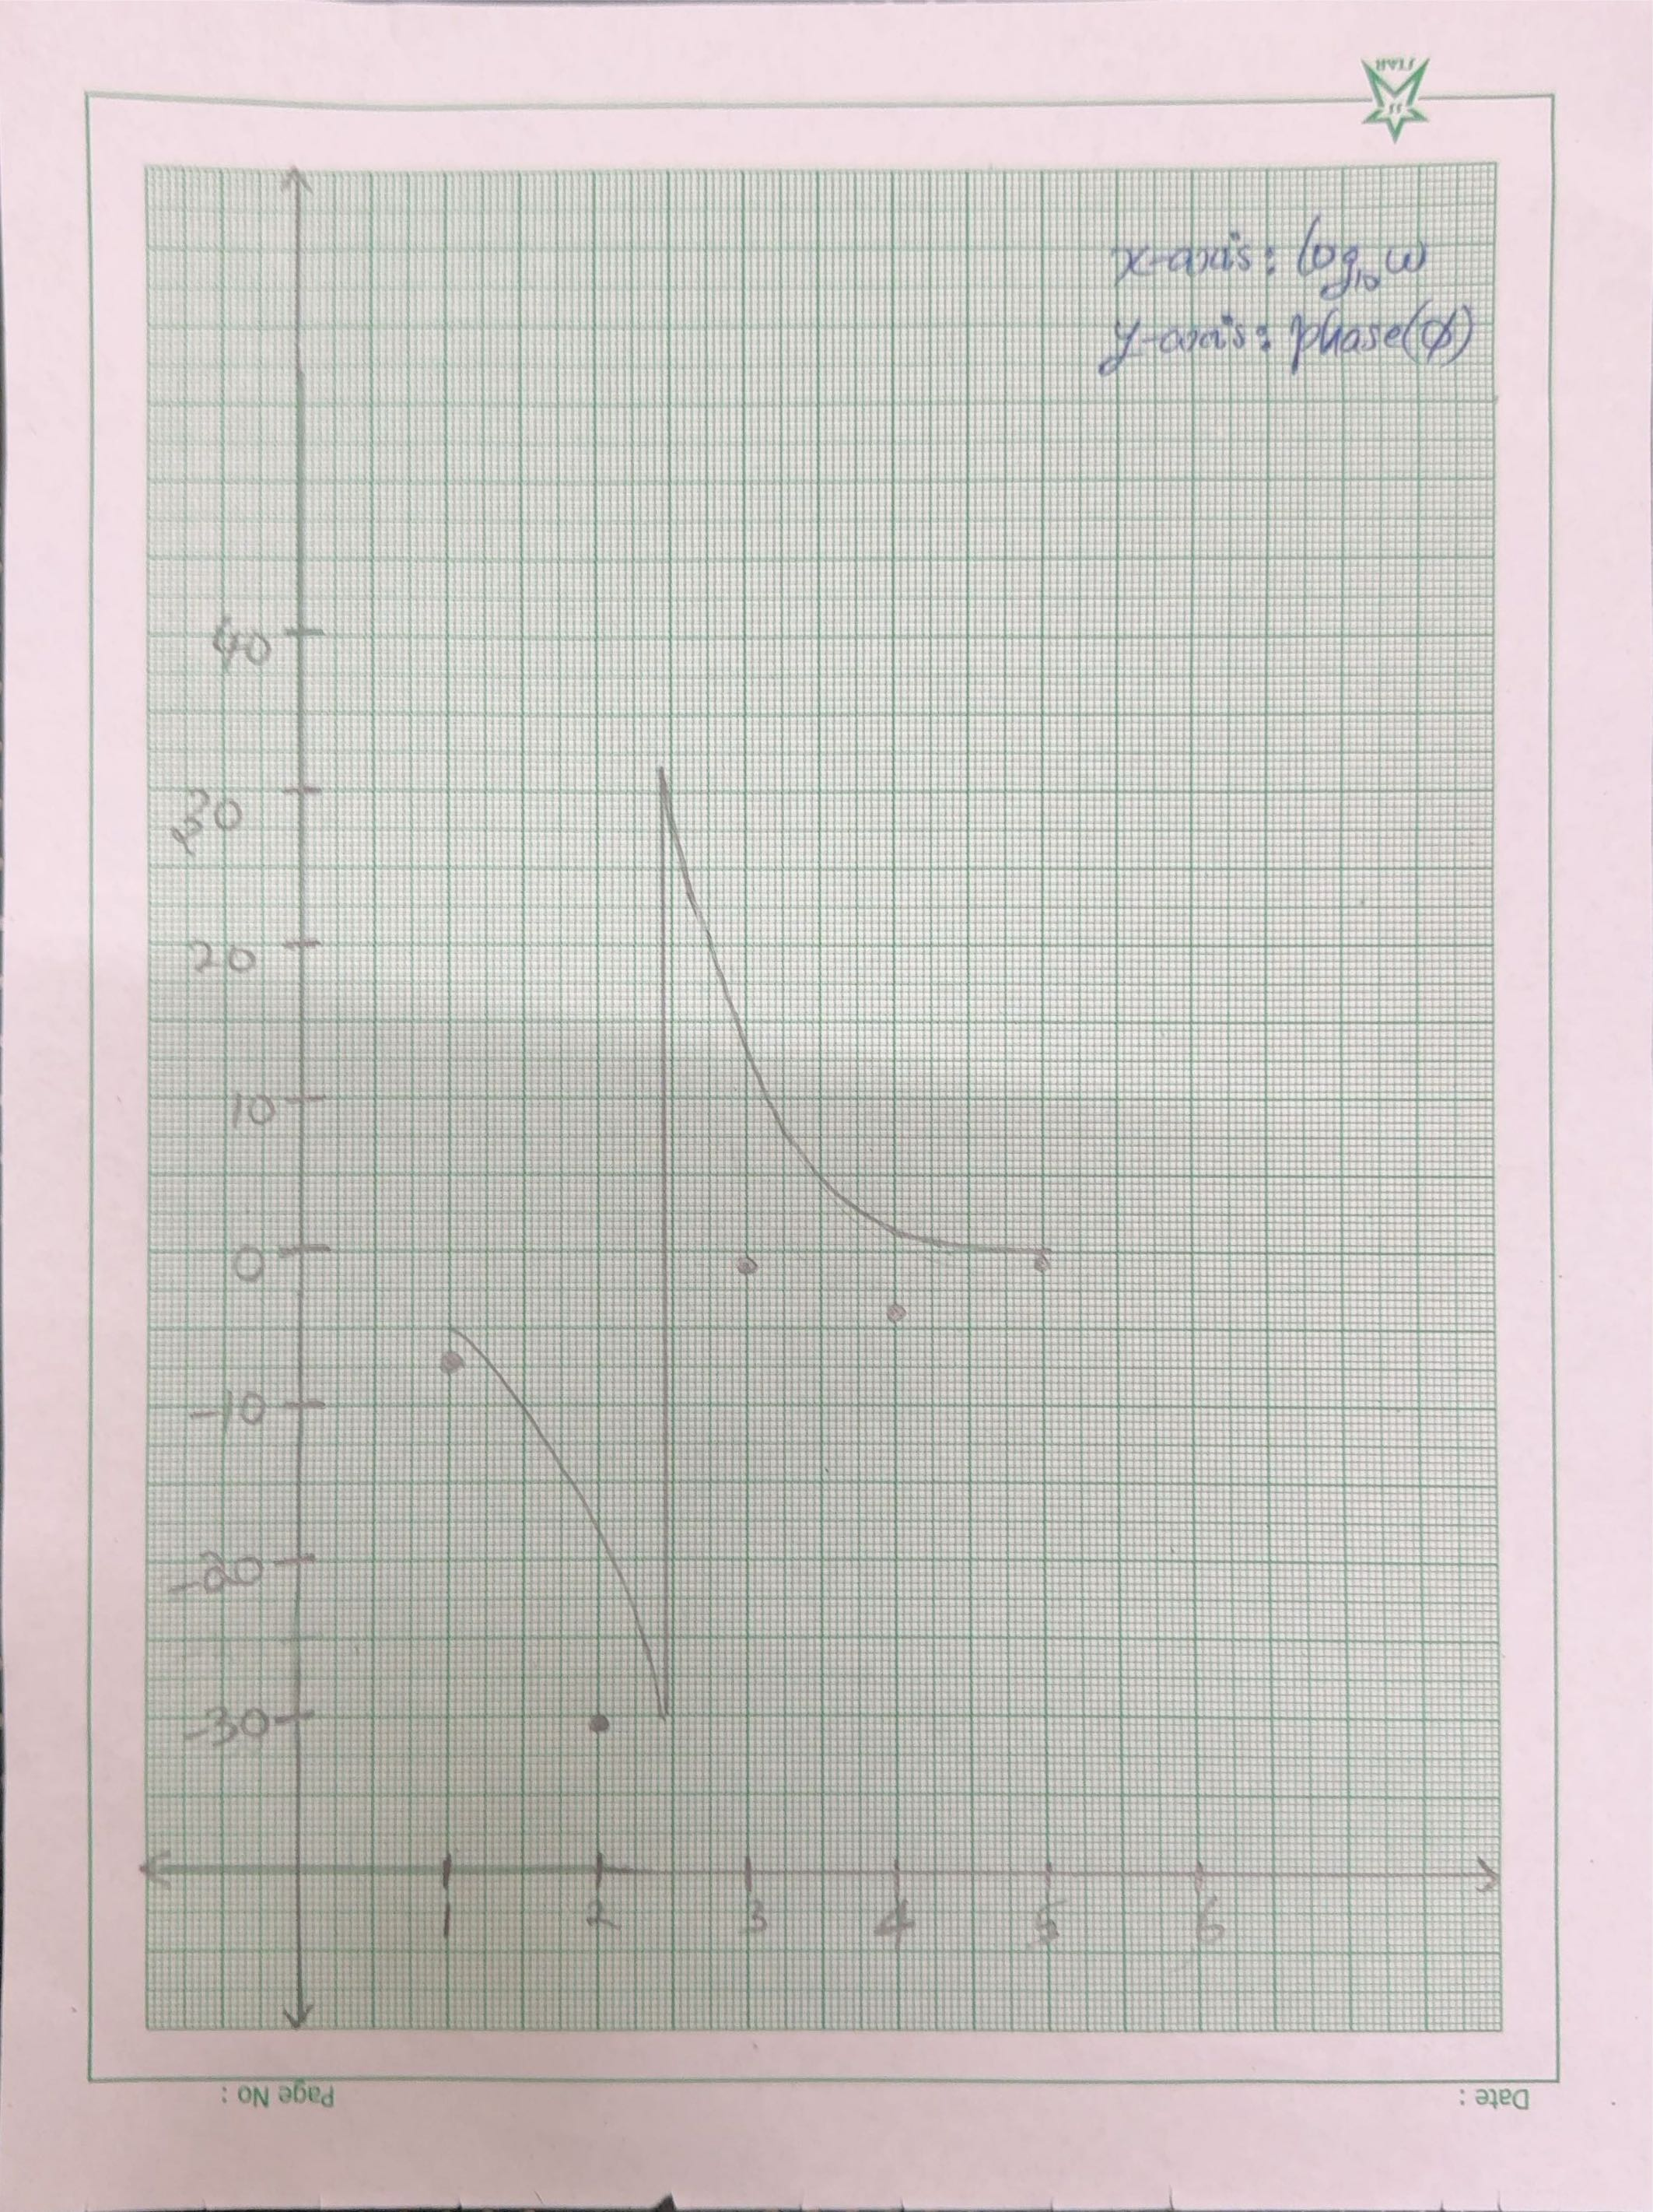
\includegraphics[width=\textwidth]{figs/phase2.png}
    \end{subfigure}
    \hfill
    \begin{subfigure}[b]{0.45\textwidth}
        \centering
        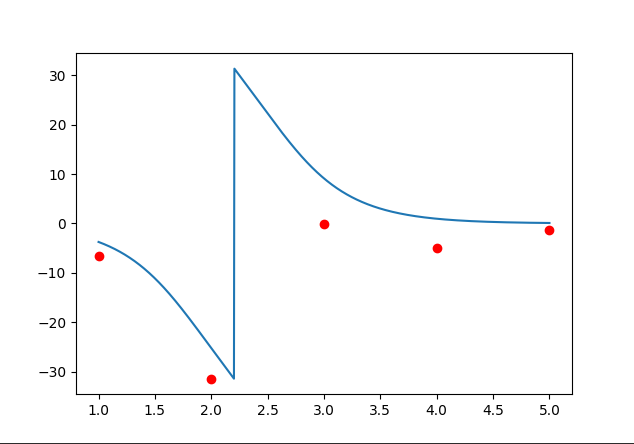
\includegraphics[width=1.7\textwidth]{figs/phase_2cas.png}
    \end{subfigure}
    
    \caption{Phase Plot for 2 cascaded RC circuit}
\end{figure}

\begin{figure}[H]
    \centering
    \begin{subfigure}[b]{0.45\textwidth}
        \centering
        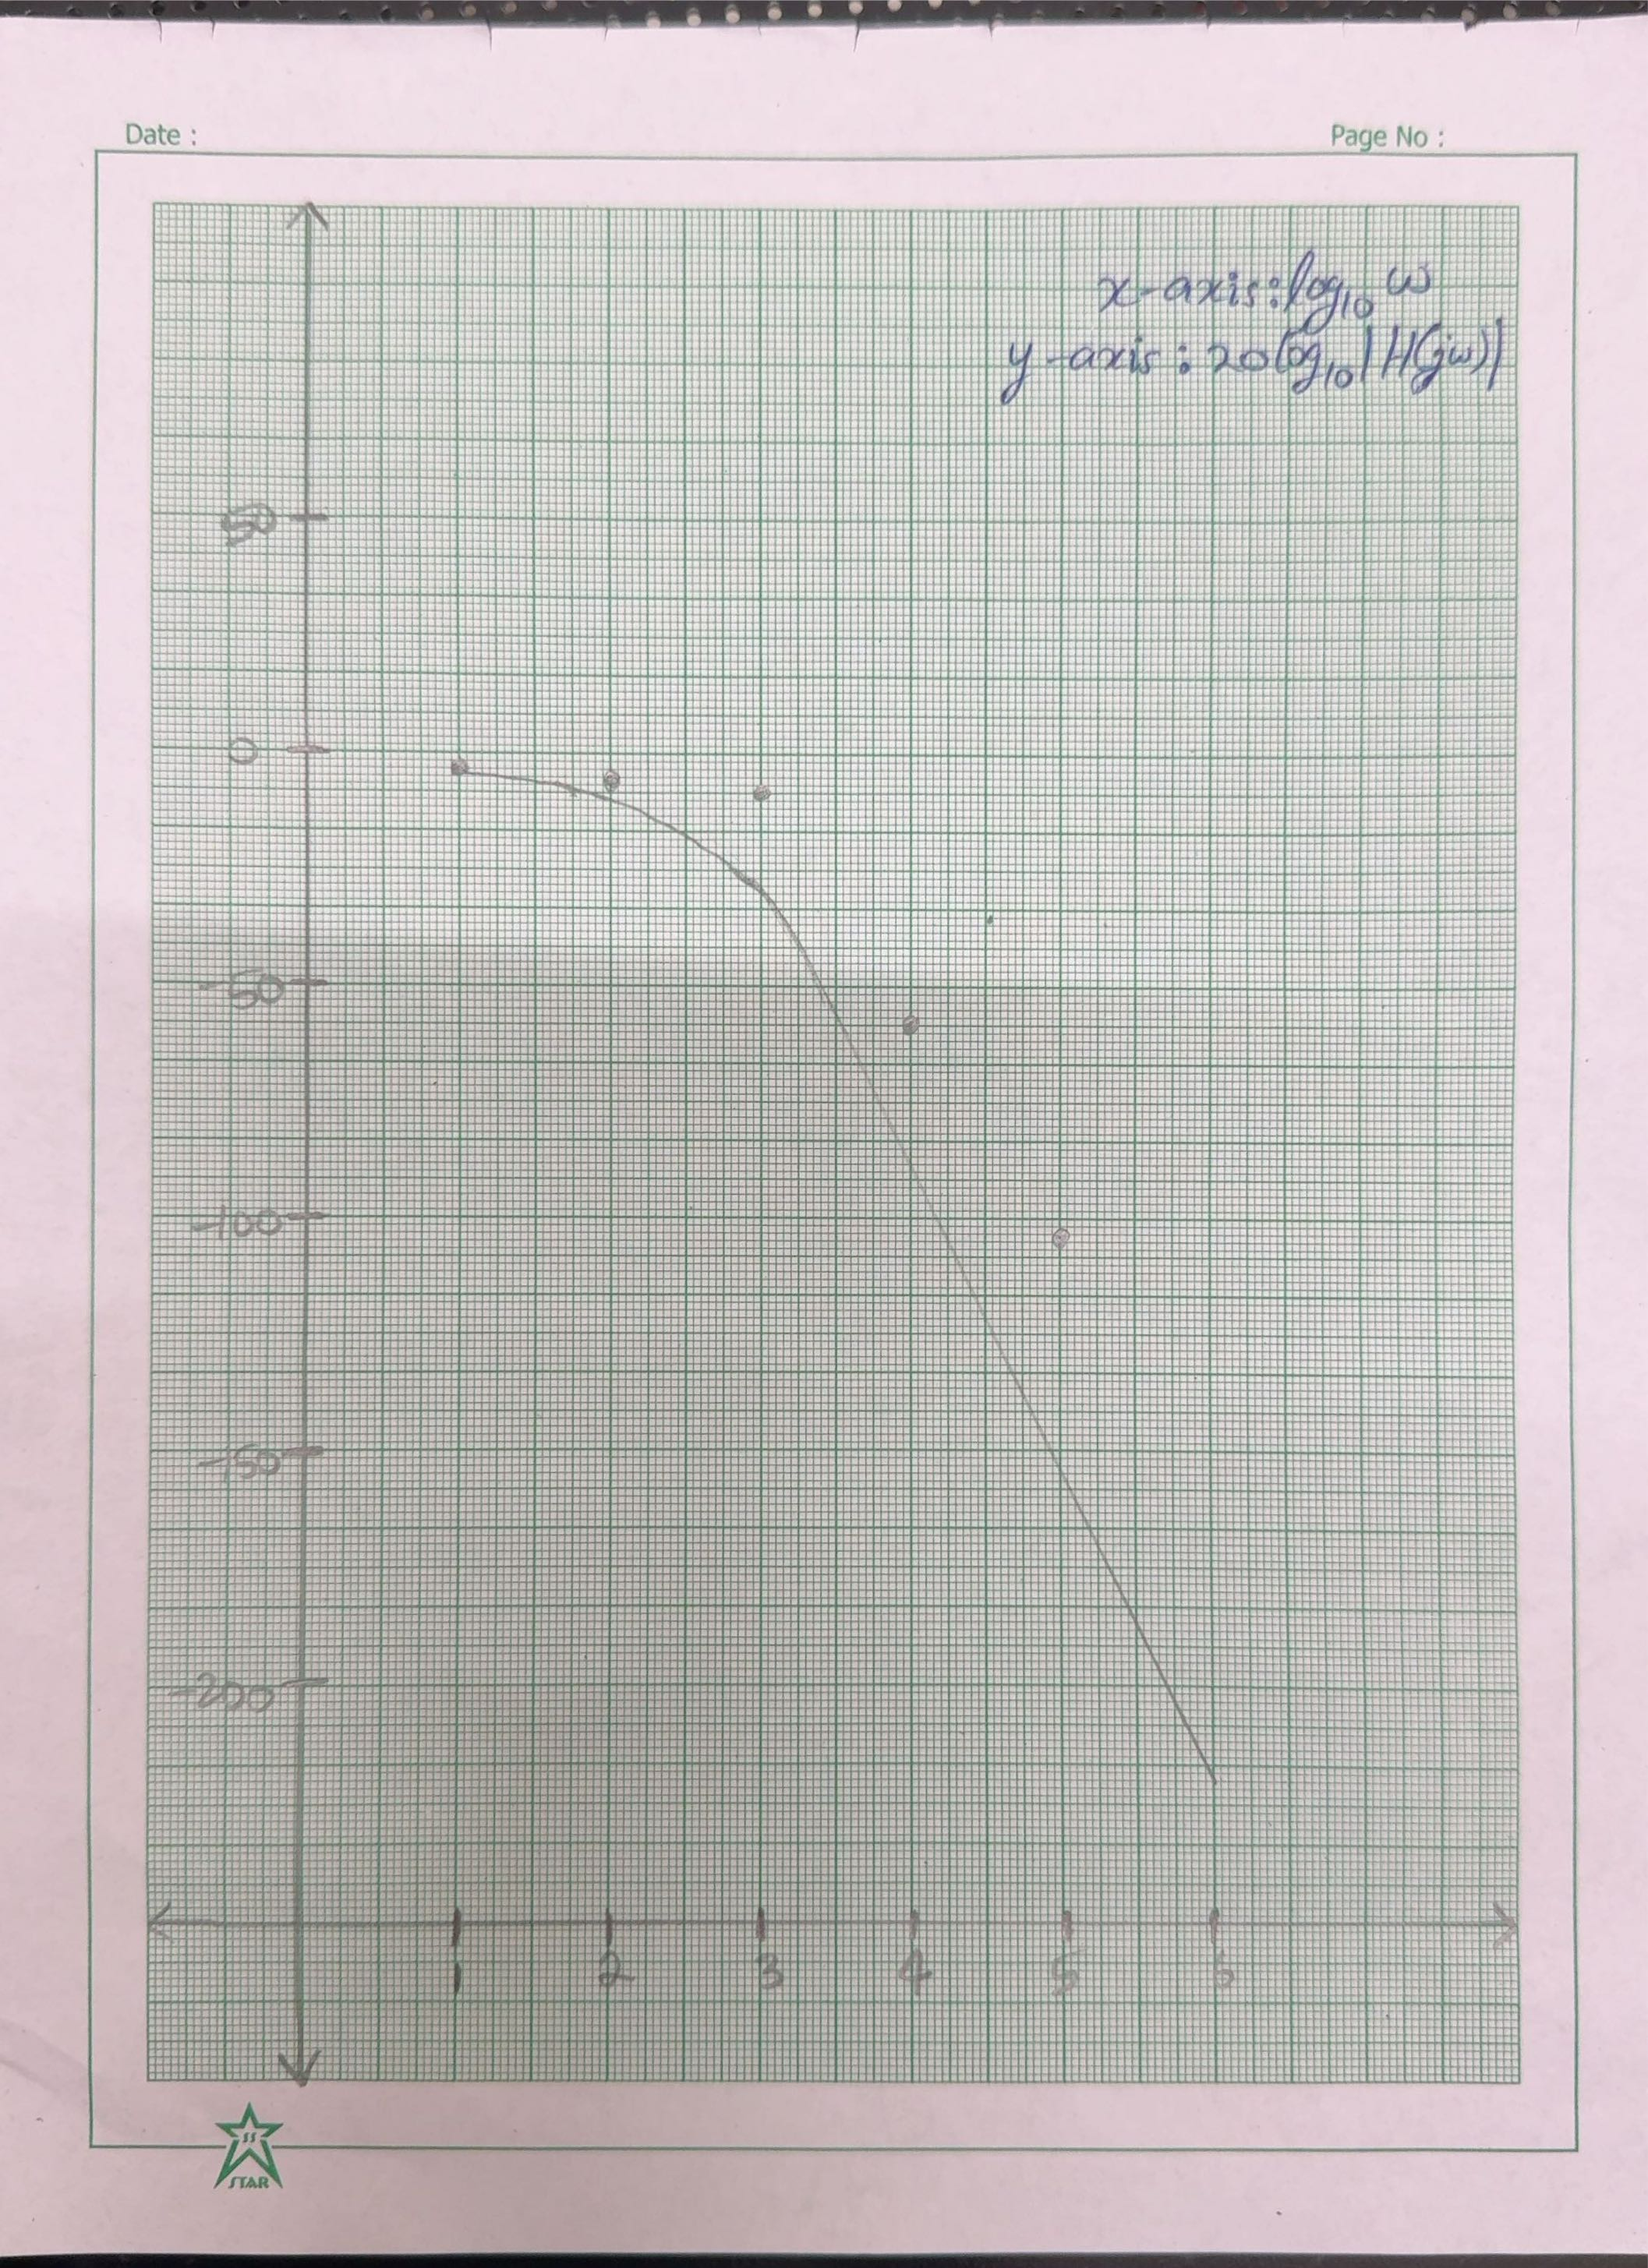
\includegraphics[width=\textwidth]{figs/ampl3.png}

    \end{subfigure}
    \hfill
    \begin{subfigure}[b]{0.45\textwidth}
        \centering
        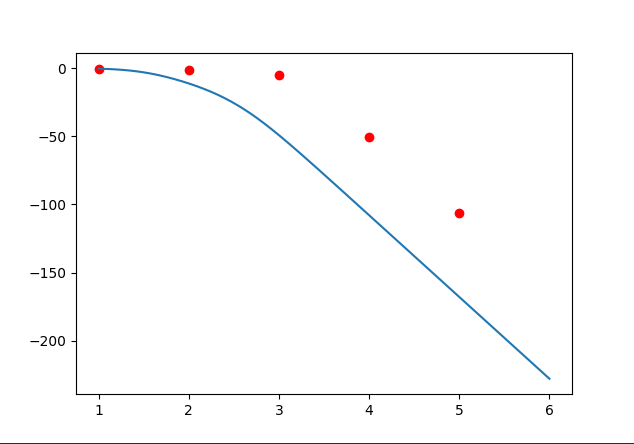
\includegraphics[width=1.7\textwidth]{figs/ampl_3cas.png}
    \end{subfigure}
    
    \caption{Amplitude Plot for 3 cascaded RC circuit}
\end{figure}

\begin{figure}[H]
    \centering
    \begin{subfigure}[b]{0.45\textwidth}
        \centering
        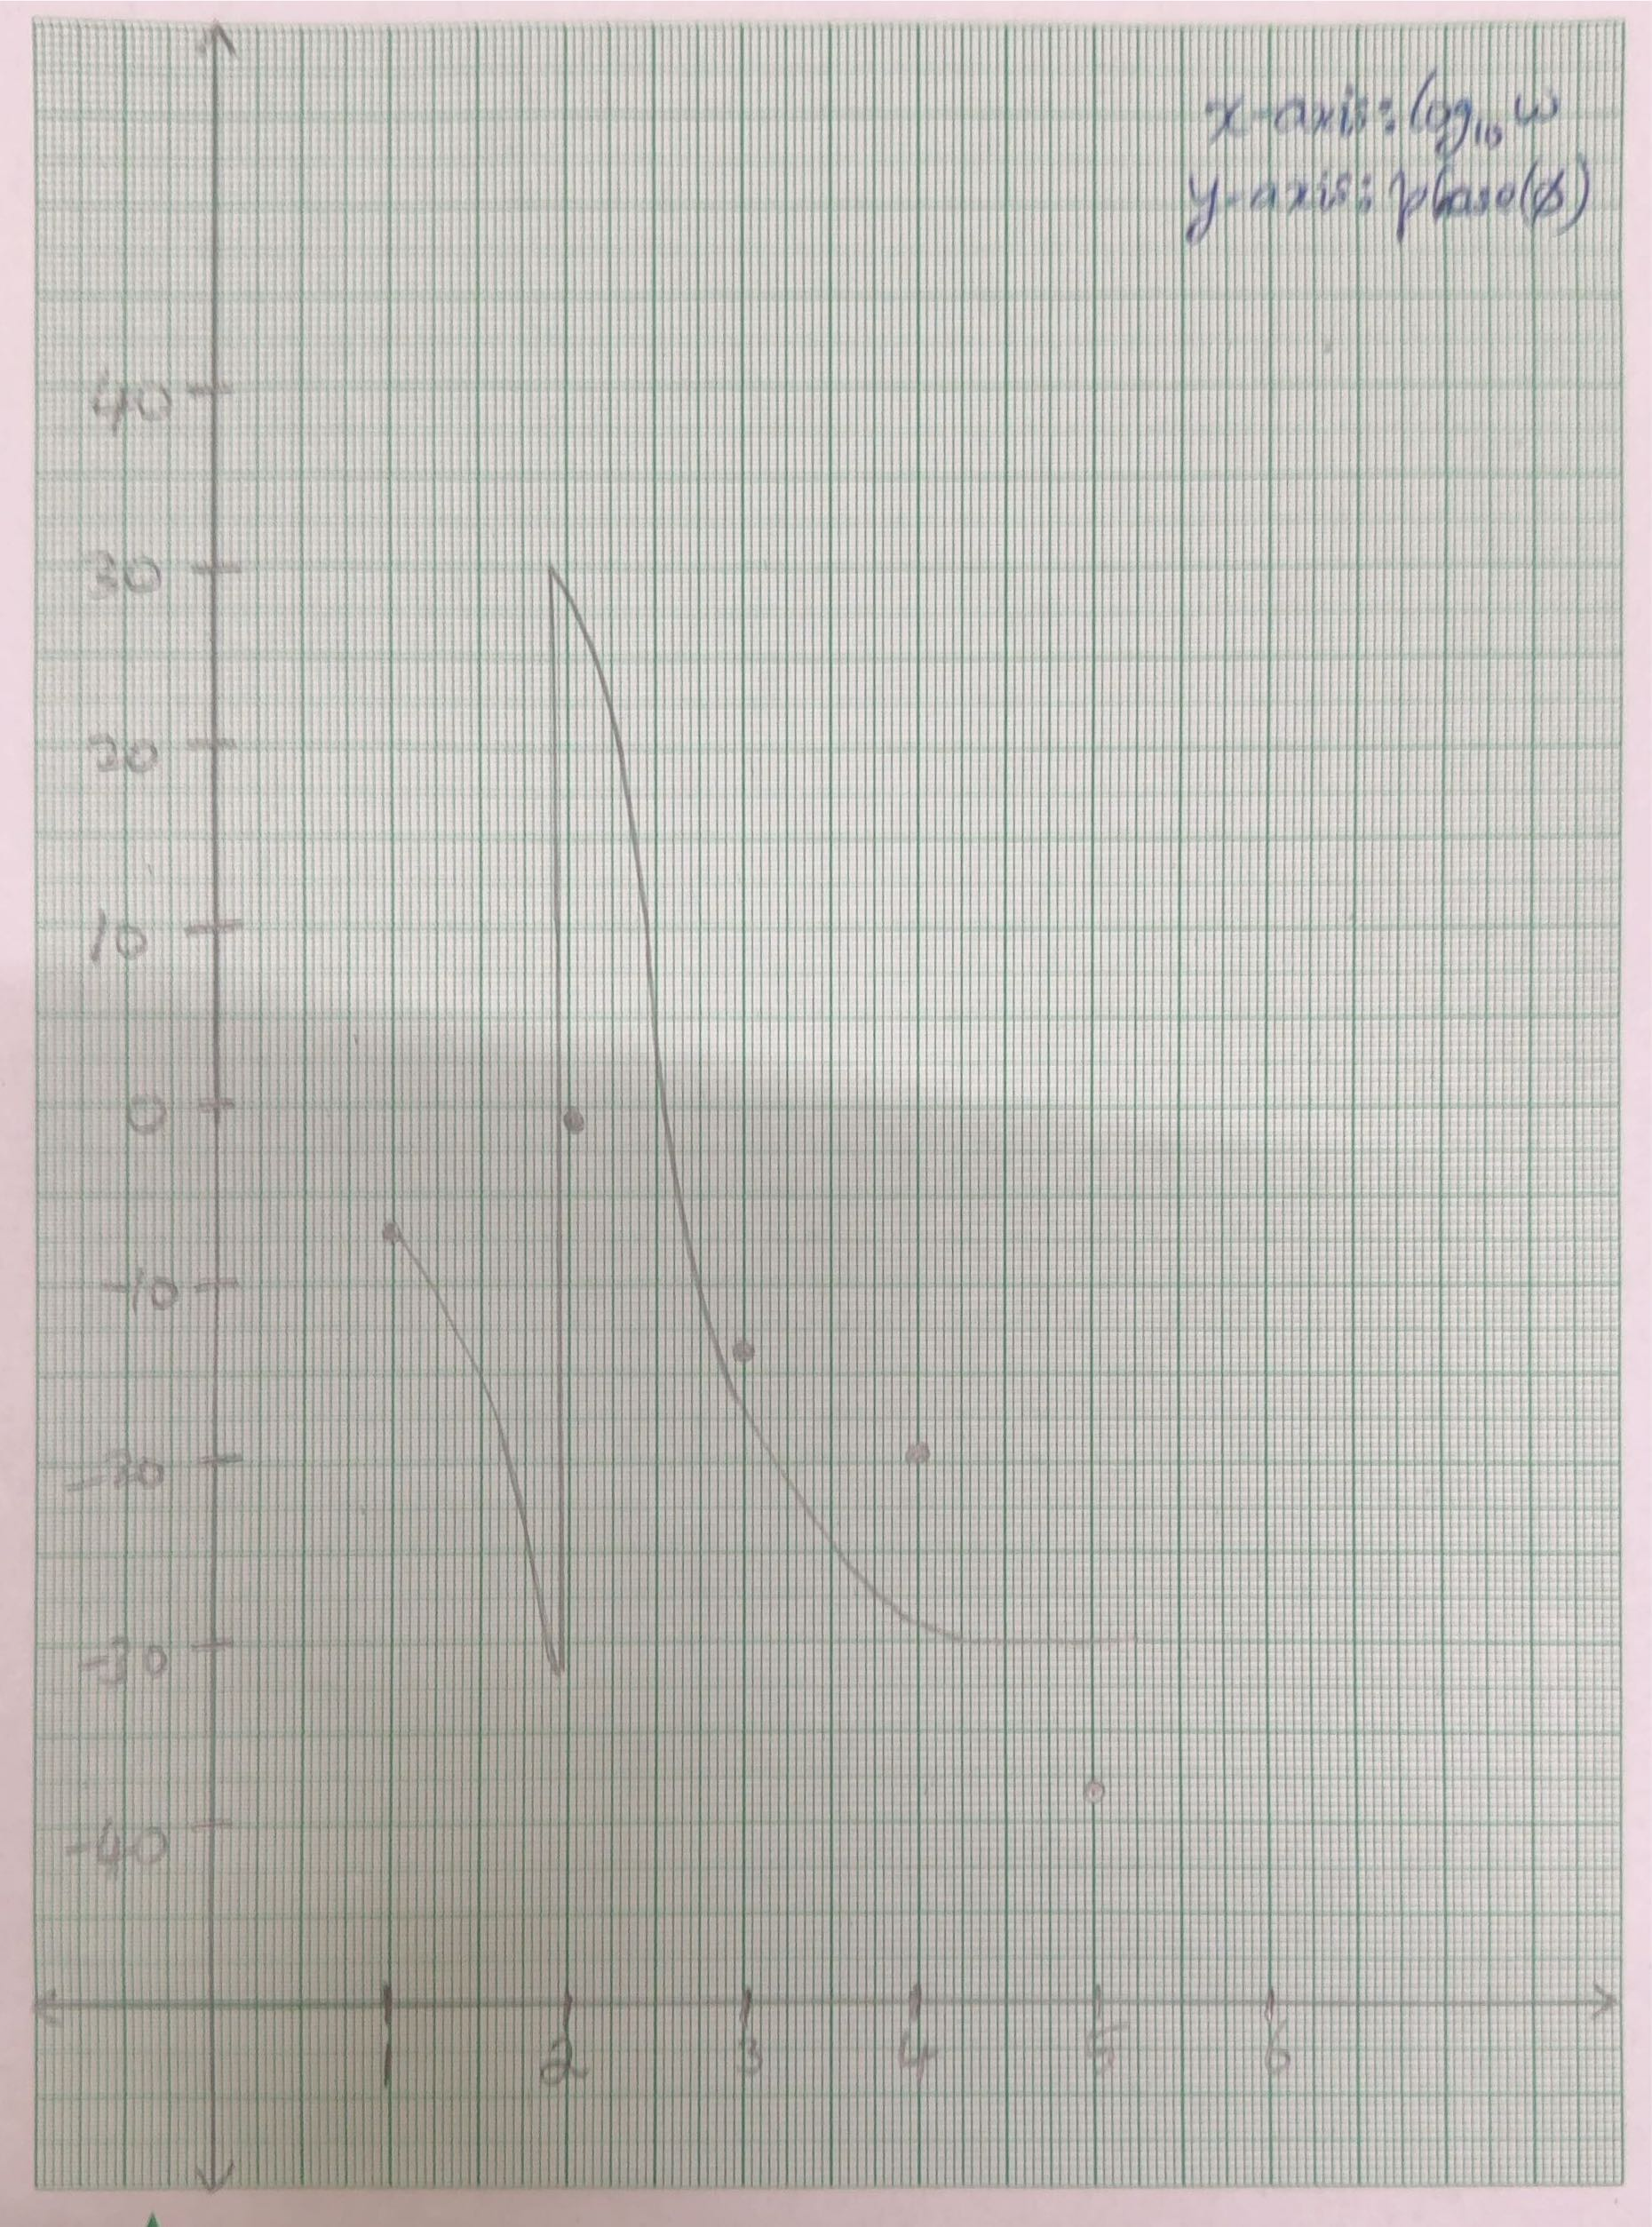
\includegraphics[width=\textwidth]{figs/phase3.png}
    \end{subfigure}
    \hfill
    \begin{subfigure}[b]{0.45\textwidth}
        \centering
        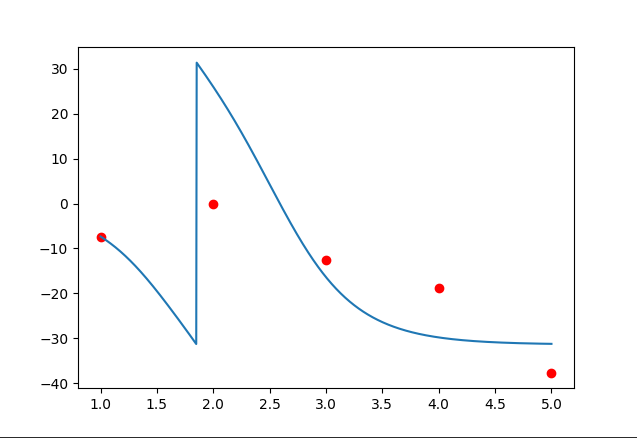
\includegraphics[width=1.7\textwidth]{figs/phase_3cas.png}
    \end{subfigure}
    
    \caption{Phase Plot for 3 cascaded RC circuit}
\end{figure}

\section{Additional Points}
\subsection{Applications of Bode Plots}
\begin{itemize}
    \item Used in circuit design to analyze frequency response.
    \item Helps in stability analysis of control systems.
    \item Used in audio and communication system filters.
\end{itemize}

\subsection{Improvements in Experimentation}
\begin{itemize}
    \item Use precision components to reduce error.
    \item Implement automated data logging for accuracy.
    \item Consider using a higher-resolution oscilloscope.
\end{itemize}
\section{Conclusion}
Cascaded RC low-pass filters provide improved attenuation characteristics by increasing the roll-off rate with each additional stage. These filters are useful in various applications, including audio processing and signal conditioning.

\end{document}
